\documentclass[11pt,a4paper]{article}

% inputenc not needed on UTF-8 engines (XeLaTeX/LuaLaTeX, modern pdfLaTeX); drop to silence warning
% \usepackage[utf8]{inputenc}
\usepackage{lmodern}
\usepackage[T1]{fontenc}
\usepackage{amsmath,amssymb,amsfonts}
\usepackage{booktabs}
\usepackage{array}
\usepackage{xcolor}
\usepackage{tikz}
\usetikzlibrary{arrows.meta,positioning,shapes.geometric}
\usepackage{graphicx}
\usepackage{geometry}
\geometry{margin=2.5cm}
\usepackage{float}
\usepackage{enumitem}
\usepackage[hidelinks,pdfencoding=auto]{hyperref}
\usepackage{algorithm}
\usepackage{algorithmic}
\usepackage{caption}
\captionsetup{hypcap=false}  % \captionof inside minipage can't anchor hypcap; silence the warning
\usepackage{subcaption}
\usepackage{multirow}

% Compact spacing
\usepackage{setspace}
\setstretch{1.08}
\setlength{\emergencystretch}{3em}  % absorb occasional overfull \hbox without \sloppy

\newcommand{\btheta}{\boldsymbol{\theta}}
\newcommand{\bphi}{\boldsymbol{\phi}}
\newcommand{\bpsi}{\boldsymbol{\psi}}
\newcommand{\yobs}{\mathbf{y}_{\mathrm{obs}}}
\newcommand{\Real}{\mathbb{R}}

\title{GPU-accelerated Bayesian inference of multi-species\\biofilm interaction parameters via TMCMC}

% Add this in your preamble (before \begin{document})
\usepackage{authblk}
\renewcommand\Affilfont{\small} % Makes affiliations slightly smaller

% Document body
\author[1]{Keisuke Nishioka}
\author[1]{Felix Klempt}
\author[1]{Hendrik Geisler}
\author[1]{Meisam Soleimani}
\author[2, 3]{Nils Heine}
\author[2, 3]{Katharina Doll-Nikutta}
\author[2, 3]{Rumjhum Mukherjee}
\author[2, 3]{Szymon P. Szafra\'{n}ski}
\author[2, 3]{Meike Stiesch}
\author[1]{Philipp Junker}

\affil[1]{Institute of Continuum Mechanics, Leibniz Universit\"at Hannover, Hannover, Germany}
\affil[2]{Department of Prosthetic Dentistry and Biomedical Materials Science, Hannover Medical School, Hannover, Germany}
\affil[3]{Lower Saxony Centre for Biomedical Engineering, Implant Research and Development (NIFE), Hannover, Germany}

\date{}

\begin{document}

\maketitle

\begin{abstract}
We present a GPU-accelerated Bayesian framework for inferring the interaction parameters of a five-species oral biofilm model derived from the extended Hamilton principle.
The symmetric $5\times5$ interaction matrix is parametrised as a 15-dimensional vector encoding 15 independent interaction coefficients.
A two-phase estimation strategy is employed: in Phase~1, the viability fraction $\psi_i$ is fixed to experimentally measured membrane-intact ratios (fix-$\psi$), enabling rapid identification of the interaction matrix; in Phase~2, $\psi_i$ is released and the viability data enter the likelihood as a soft constraint, yielding a self-consistent posterior over both interactions and viability.
The forward model is compiled via JAX and evaluated in parallel on GPU (NVIDIA RTX\,4090), achieving a $\sim$200$\times$ speedup over the CPU baseline.
No interaction parameters are locked to zero a priori; the posterior self-organises, concentrating pathogen-related entries near zero in commensal conditions and activating cooperative cross-feeding terms in dysbiotic states.
The method is validated against in-vitro time-course data from Heine et al.\ under four combinations of community state (commensal/dysbiotic) and cultivation mode (static/HOBIC reactor).

\vspace{4pt}
\noindent\textbf{Keywords:}
Bayesian inference,
biofilm dynamics,
TMCMC,
GPU acceleration,
parameter identification,
multi-species interaction,
peri-implantitis
\end{abstract}

%==============================================================================
\section{Introduction}
\label{sec:intro}
%==============================================================================

Multi-species biofilms that form on dental implant surfaces are a principal etiological factor in peri-implantitis~\cite{Kolenbrander2010OralMultispecies, Marsh2003Dental}. Recent \textit{in vivo} characterisations indicate that these microbial communities are highly complex, individualized, and dynamically structured over time~\cite{EarlyImplantBiofilm2024, PeriImplantitisDysbiosis2025}.
In a controlled in vitro study, Heine et al.~\cite{Heine2025PeriImplant} investigated the temporal dynamics of five representative oral taxa, \textit{Streptococcus oralis} (\textit{So}), \textit{Actinomyces naeslundii} (\textit{An}), \textit{Veillonella} spp.\ (\textit{Vei}), \textit{Fusobacterium nucleatum} (\textit{Fn}), and \textit{Porphyromonas gingivalis} (\textit{Pg}), across four experimental conditions defined by community state (commensal vs. dysbiotic) and cultivation mode (static vs. HOBIC reactor).
Importantly, the two community states incorporated distinct \textit{Porphyromonas gingivalis} strains: the commensal consortium included the avirulent strain \textit{Pg} ATCC 20709, whereas the dysbiotic consortium employed the virulent strain \textit{Pg} W83, which harbors a full complement of gingipain and fimbrial virulence determinants~\cite{Heine2025PeriImplant}.
Building on the extended Hamilton principle~\cite{JunkerBalzani2021ExtendedHamilton}, Klempt et al.~\cite{Klempt2025ContinuumBiofilm} formulated a continuum model in which a symmetric interaction matrix~$\mathbf{A}$ governs species growth, with an optional decay vector~$\mathbf{b}$ for antibiotic effects.
Fritsch et al.~\cite{Fritsch2025BayesianMicrofilms} subsequently introduced Bayesian updating with surrogate models for biofilm parameter estimation under hybrid uncertainties.

Despite these advances, estimating the 15-dimensional parameter vector (15 interaction parameters) from limited time-course data remains challenging.
Two principal difficulties arise: (i) poor identifiability when data are sparse relative to the parameter dimension---with $N_t=5$ usable time points (Day~1 is consumed as initial condition) and 5 species, one has at most 25 observations for 15 unknowns---and (ii) multimodal posterior landscapes caused by the coupled $\phi_i$--$\psi_i$ dynamics, which render standard MCMC methods inefficient~\cite{RobertCasella2004MonteCarlo}.

In this work we address these challenges through three complementary strategies.
First, we fix the viability fraction $\psi_i$ to experimentally measured membrane-intact ratios, eliminating $\psi$-related posterior modes and halving the ODE system dimension.
Second, we compile the forward model in JAX~\cite{jax2018github} and evaluate the entire particle ensemble on GPU via batched \texttt{vmap}, achieving a $\sim$200$\times$ speedup over the CPU baseline.
Third, we employ iteratively narrowed priors that concentrate sampling on the high-posterior-density region, enabling convergence in 5--7 TMCMC~\cite{ChingChen2007TMCMC, Betz2016TMCMC} stages even in 15 dimensions.
The framework is validated against all four experimental conditions of Heine et al., demonstrating quantitative reproduction of commensal homeostasis as well as the non-linear pathogen surge characteristic of dysbiotic biofilms under HOBIC flow.

%==============================================================================
\section{Mathematical model}
\label{sec:model}
%==============================================================================

\subsection{State variables and kinematics}

Following Klempt et al.~\cite{Klempt2025ContinuumBiofilm, Klempt2024ContinuumGrowth}, the biofilm is described at a material point by two sets of internal variables: the volume fraction $\phi_i \in [0,1]$ occupied by species~$i$ ($i=1,\dots,n$; here $n=5$), and the viability fraction $\psi_i \in [0,1]$ representing the proportion of living cells within species~$i$.
The living volume fraction is then
\begin{equation}
\bar{\phi}_i := \phi_i\,\psi_i,
\qquad i=1,\dots,n.
\label{eq:living}
\end{equation}
An additional void fraction~$\phi_0$ closes the system via the holonomic constraint
\begin{equation}
\sum_{l=0}^{n}\phi_l(t) - 1 = 0 \quad\forall\,t.
\label{eq:constraint}
\end{equation}

\subsection{Variational formulation}

The evolution equations are derived from the extended Hamilton principle~\cite{JunkerBalzani2021ExtendedHamilton, JunkerBodeHackl2025Holistic}
\begin{equation}
\mathcal{H} = \int_\tau \bigl(\mathcal{G} + \mathcal{C} + \mathcal{D}\bigr)\,\mathrm{d}t \to \mathrm{stat}_{\boldsymbol{\xi},\gamma}\,,
\label{eq:hamilton}
\end{equation}
where $\boldsymbol{\xi}=(\boldsymbol{\phi},\boldsymbol{\psi})^T$ collects the volume fractions and viability fractions, $\gamma$ is a Lagrange multiplier enforcing the volume constraint, $\mathcal{G}$ is the Helmholtz free energy, $\mathcal{C}$ the constraint functional, and $\mathcal{D}$ the dissipation.
The free energy density encodes nutrient-driven growth and antibiotic-induced killing:
\begin{equation}
\Psi = -\tfrac{1}{2}\,c^*\,\bar{\bphi}^T \mathbf{A}\,\bar{\bphi}
      + \tfrac{1}{2}\,\alpha^*\,\bpsi^T \mathbf{B}\,\bpsi,
\label{eq:psi}
\end{equation}
where $c^*$ is the nutrient concentration, $\alpha^*$ the antibiotic concentration, $\mathbf{A}\in\Real^{n\times n}$ the symmetric growth coefficient matrix, and $\mathbf{B}=\mathrm{diag}(b_1,\dots,b_n)$ the antibiotic sensitivity matrix.
The volume constraint~\eqref{eq:constraint} enters through a Lagrange multiplier~$\gamma$:
\begin{equation}
\mathcal{C} = \gamma\Bigl(\sum_{l=0}^{n}\phi_l - 1\Bigr).
\label{eq:cfunc}
\end{equation}
The dissipation $\mathcal{D}$ is derived from the rate-dependent potential~\cite{Klempt2025ContinuumBiofilm}
\begin{equation}
\mathcal{D} = \tfrac{1}{2}\,\dot{\bar{\bphi}}^T\boldsymbol{\eta}\,\dot{\bar{\bphi}}
          + \tfrac{1}{2}\,\dot{\bphi}^T\boldsymbol{\eta}\,\dot{\bphi},
\label{eq:dissipation}
\end{equation}
with the diagonal viscosity matrix $\boldsymbol{\eta}=\mathrm{diag}(\eta_1,\dots,\eta_n)$.
The first term couples $\dot\phi_i$ and $\dot\psi_i$ through $\dot{\bar\phi}_i = \dot\phi_i\psi_i + \phi_i\dot\psi_i$, giving rise to non-linear dissipative interactions; the second term regularises the system to full rank.
Following Klempt et al.~\cite{Klempt2025ContinuumBiofilm}, the viscosity parameters are set to $\eta_i=1$ for all species, rendering them dimensionless scaling factors; the physical time scale is absorbed into the time-step size $\Delta t$.

\subsection{Governing equations}

Evaluating $\delta\mathcal{H}=0$ with respect to variations $\delta\phi_i$, $\delta\psi_i$, and $\delta\gamma$ yields the coupled evolution equations~\cite{Klempt2025ContinuumBiofilm}:

\medskip\noindent
\textit{Volume fraction} ($i=1,\dots,n$):
\begin{equation}
0 = -c^*\,\psi_i\,\bigl(\mathbf{A}\bar{\bphi}\bigr)_i
    + \eta_i\bigl(\dot\phi_i\,\psi_i^2 + \bar\phi_i\,\dot\psi_i + \dot\phi_i\bigr)
    + \gamma,
\label{eq:phi}
\end{equation}

\noindent\textit{Viability fraction} ($i=1,\dots,n$):
\begin{equation}
0 = -c^*\,\phi_i\,\bigl(\mathbf{A}\bar{\bphi}\bigr)_i
    + \alpha^*\,b_i\,\psi_i
    + \eta_i\bigl(\dot\psi_i\,\phi_i^2 + \bar\phi_i\,\dot\phi_i\bigr)
    + \gamma,
\label{eq:psi_evol}
\end{equation}

\noindent\textit{Void fraction}:
\begin{equation}
0 = \gamma + \dot\phi_0,
\label{eq:phi0}
\end{equation}

\noindent\textit{Volume constraint}:
\begin{equation}
0 = \sum_{l=0}^{n}\phi_l - 1,
\label{eq:constraint_eq}
\end{equation}
In the numerical implementation, a logarithmic barrier penalty $\Psi_{\mathrm{bar}}$ with $K_p=\eta_i\times10^{-4}$ is added to enforce the box constraints $\phi_i,\psi_i\in(0,1)$~\cite{Klempt2025ContinuumBiofilm}; its contribution is omitted from Eqs.~\eqref{eq:phi}--\eqref{eq:phi0} for clarity.
The system~\eqref{eq:phi}--\eqref{eq:constraint_eq} constitutes $2n+2$ coupled non-linear equations for the unknowns $(\phi_1,\dots,\phi_n,\phi_0,\psi_1,\dots,\psi_n,\gamma)$, solved at each time step via Newton's method with an implicit Euler discretisation ($\Delta t = 10^{-4}$, $N_t=2{,}500$ steps, $t_{\max}=0.25$ corresponding to the 21-day experimental window).

The variational derivation automatically ensures symmetry $A_{ij}=A_{ji}$ and thermodynamic consistency~\cite{JunkerBalzani2021ExtendedHamilton}.
Since $c^*$ enters the evolution equations only through the product $c^*A_{ij}$, its absolute value is non-identifiable; we fix $c^*=25$ so that the inferred $A_{ij}$ remain $\mathcal{O}(1)$.
The Heine et al.\ experiments do not involve antibiotic agents, so we set $\alpha^*=0$, which eliminates the decay term $\alpha^*b_i\psi_i$ from Eq.~\eqref{eq:psi_evol}; the antibiotic sensitivity matrix~$\mathbf{B}$ is therefore inactive and excluded from estimation.
The symmetric interaction matrix~$\mathbf{A}$ has 15 independent entries(Section~\ref{sec:model_matrix}), these form the 15-dimensional parameter vector~$\btheta$.

\subsection{Symmetric interaction matrix}
\label{sec:model_matrix}

The symmetry $A_{ij}=A_{ji}$ arises automatically from the quadratic form of the free energy~\eqref{eq:psi}, reducing the off-diagonal degrees of freedom from 20 to~10.
Together with the 5 diagonal entries, the symmetric matrix has 15 independent entries.
These are distinct from the antibiotic sensitivity parameters~$b_i$ in Eq.~\eqref{eq:psi_evol}, which vanish when $\alpha^*=0$.
The resulting 15-dimensional parameter vector is
\begin{equation}
\btheta = (\theta_0,\dots,\theta_{14})^T \in \Real^{15},
\label{eq:theta}
\end{equation}
organised into five biologically motivated blocks:
\begin{equation}
\btheta =
\underbrace{(a_{11},a_{12},a_{22})}_{\text{So--An}}
\oplus
\underbrace{(a_{33},a_{34},a_{44})}_{\text{Vei--Fn}}
\oplus
\underbrace{(a_{13},a_{14},a_{23},a_{24})}_{\text{cross}}
\oplus
\underbrace{(a_{15},a_{25},a_{35},a_{45})}_{\text{Pg cross}}
\oplus
\underbrace{(a_{55})}_{\text{Pg}}.
\label{eq:blocks}
\end{equation}

\subsection{Biological interaction network}

The interaction network reported by Heine et al.~\cite{Heine2025PeriImplant} comprises five experimentally validated species pairs (Figure~\ref{fig:network}).
 For an additional five pairs, no direct metabolic exchange or co-aggregation mechanisms have been described. Rather than imposing these absences as hard constraints (i.e., $\theta_k\equiv0$), we estimate the full set of 15 interaction parameters and allow the posterior distribution to infer which interactions are supported by the data.

This framework is made computationally tractable by the fix-$\psi$ strategy (Section~\ref{sec:gpu}), which mitigates posterior multimodality and enables stable convergence in the 15-dimensional parameter space.

\begin{figure}[htbp]
\centering
\begin{minipage}[t]{0.32\textwidth}
\vspace{0pt}
\centering
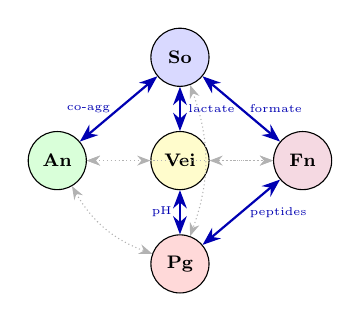
\begin{tikzpicture}[scale=0.82, every node/.style={transform shape},
    species/.style={circle, draw, minimum size=0.9cm, font=\footnotesize\bfseries},
    edge/.style={<->, thick, >=Stealth},
    weakedge/.style={<->, thin, gray!60, >=Stealth, densely dotted}
]
    \node[species, fill=blue!15] (so) at (0, 2.2) {So};
    \node[species, fill=green!15] (an) at (-1.9, 0.6) {An};
    \node[species, fill=yellow!20] (vei) at (0, 0.6) {Vei};
    \node[species, fill=purple!15] (fn) at (1.9, 0.6) {Fn};
    \node[species, fill=red!15] (pg) at (0, -1.0) {Pg};
    \draw[edge, blue!70!black] (so) -- (an) node[midway, left, font=\tiny] {co-agg};
    \draw[edge, blue!70!black] (so) -- (vei) node[midway, right, font=\tiny] {lactate};
    \draw[edge, blue!70!black] (so) -- (fn) node[midway, right, font=\tiny] {formate};
    \draw[edge, blue!70!black] (vei) -- (pg) node[midway, left, font=\tiny] {pH};
    \draw[edge, blue!70!black] (fn) -- (pg) node[midway, right, font=\tiny] {peptides};
    \draw[weakedge] (an) -- (vei);
    \draw[weakedge] (an) -- (fn);
    \draw[weakedge] (vei) -- (fn);
    \draw[weakedge] (so) to[bend left=20] (pg);
    \draw[weakedge] (an) to[bend right=20] (pg);
\end{tikzpicture}
\end{minipage}%
\hfill
\begin{minipage}[t]{0.65\textwidth}
\vspace{0pt}
\small
\begin{tabular}{@{}lll@{}}
\toprule
\textbf{Pair} & \textbf{Mechanism} & \textbf{Type}\\
\midrule
So--An & Co-aggregation & Bidirectional\\
So--Vei & Lactate exchange & Bidirectional\\
So--Fn & Formate symbiosis & Bidirectional\\
Vei$\to$Pg & pH elevation & Unidirectional\\
Fn--Pg & Peptide supply & Bidirectional\\
\bottomrule
\end{tabular}
\captionof{table}{Experimentally confirmed species interactions~\cite{Heine2025PeriImplant}. All 15 parameters are estimated without a priori locking; the posterior concentrates near zero for biologically inactive pairs.}
\label{tab:active}
\end{minipage}
\caption{Species interaction network~\cite{Heine2025PeriImplant}. Solid blue: experimentally confirmed pathways. Dotted grey: no known pathway, estimated freely---the posterior determines their magnitude.}
\label{fig:network}
\end{figure}

The block symbols $a_{ij}$ follow the 1-based notation of Klempt et al.~\cite{Klempt2025ContinuumBiofilm}; the matrix entries $A_{ij}$ use 0-based indexing consistent with Eqs.~\eqref{eq:phi}--\eqref{eq:psi_evol}.

%==============================================================================
\section{Bayesian inference framework}
\label{sec:bayes}
%==============================================================================

\subsection{Posterior distribution}

Given observed time-course data $\yobs = \{y_{\mathrm{obs},i}(t_k)\}$, we seek the posterior
\begin{equation}
p(\btheta\mid\yobs)
= \frac{p(\yobs\mid\btheta)\,p(\btheta)}{p(\yobs)},
\label{eq:bayes}
\end{equation}
where $p(\yobs\mid\btheta)$ is the likelihood, $p(\btheta)$ the prior, and $p(\yobs)$ the model evidence.

\subsection{Likelihood}

Assuming independent Gaussian errors across species and time points:
\begin{equation}
p(\yobs\mid\btheta)
= \prod_{k=1}^{N_t}\prod_{i=0}^{4}
\frac{1}{\sqrt{2\pi}\,\sigma_{i}}
\exp\!\Bigl(-\frac{(y_{\mathrm{obs},i}(t_k)-\hat{y}_i(t_k;\btheta))^2}{2\sigma_{i}^2}\Bigr),
\label{eq:likelihood}
\end{equation}
where $\sigma_{i}$ is a species-specific observation noise derived from the replicate standard deviation of the normalised species fractions at each time point~\cite{Heine2025PeriImplant} ($N=8$ biological replicates per condition).
The noise is averaged over time points to yield a fixed $\sigma_i$ per species per condition, with typical values ranging from $\sigma_i\approx0.05$ (\textit{Fn}, \textit{Pg} in commensal states where fractions are near zero) to $\sigma_i\approx0.20$ (\textit{So} in commensal states where variability is highest).
The condition-averaged mean noise is $\bar{\sigma}\approx0.11$--$0.12$ across all conditions.

\subsection{Constrained prior}

The prior is a product of independent uniform distributions:
\begin{equation}
p(\btheta) = \prod_{k=0}^{19} \frac{1}{u_k-l_k}\,\mathbf{1}_{[l_k,u_k]}(\theta_k),
\label{eq:prior}
\end{equation}
where the bounds $[l_k,u_k]$ are condition-specific and iteratively narrowed (Section~\ref{sec:gpu}).
All 15 parameters are estimated for every condition; no parameters are locked to zero a priori.
The prior bounds are initialised broadly ($[l_k,u_k]\approx[-1,1]$ for most parameters) and refined after an initial TMCMC run using the posterior quantile range plus $1.5\sigma$ padding.

%==============================================================================
\section{TMCMC inference}
\label{sec:tmcmc}
%==============================================================================

\subsection{Tempered likelihood sequence}

TMCMC~\cite{ChingChen2007TMCMC, DelMoral2006SMC, Chopin2002SMC} constructs a sequence of intermediate distributions
\begin{equation}
p_m(\btheta) \propto p(\yobs\mid\btheta)^{\beta_m}\,p(\btheta),
\qquad
0=\beta_0<\beta_1<\cdots<\beta_M=1,
\label{eq:tempered}
\end{equation}
interpolating from the prior ($\beta_0=0$) to the full posterior ($\beta_M=1$).
The tempering parameter $\beta_{m+1}$ is determined adaptively so that the coefficient of variation of the importance weights
\begin{equation}
w_j^{(m)} = p(\yobs\mid\btheta_j^{(m)})^{\beta_{m+1}-\beta_m},
\qquad j=1,\dots,N,
\label{eq:weights}
\end{equation}
satisfies $\mathrm{CoV}[\{w_j^{(m)}\}]=\delta_{\mathrm{target}}$, solved by bisection on $(\beta_m,1]$~\cite{Betz2016TMCMC}.

\subsection{Resampling and mutation}

At each stage~$m$:
\begin{enumerate}[nosep,leftmargin=*]
\item \textbf{Resample} $N$ particles from $\{\btheta_j^{(m)}\}$ with probabilities $\propto w_j^{(m)}$.
\item \textbf{Estimate} the weighted covariance
\begin{equation}
\boldsymbol{\Sigma}^{(m)}
= \sum_{j=1}^{N}\bar{w}_j^{(m)}
\bigl(\btheta_j^{(m)}-\bar{\btheta}^{(m)}\bigr)
\bigl(\btheta_j^{(m)}-\bar{\btheta}^{(m)}\bigr)^T.
\label{eq:cov}
\end{equation}
\item \textbf{Mutate} each particle via Metropolis--Hastings with proposal $q(\btheta^*\mid\btheta_j)=\mathcal{N}(\btheta_j,\gamma^2\boldsymbol{\Sigma}^{(m)})$ and acceptance probability
\begin{equation}
\alpha = \min\!\biggl(1,\;
\frac{p(\yobs\mid\btheta^*)^{\beta_{m+1}}\,p(\btheta^*)}
     {p(\yobs\mid\btheta_j)^{\beta_{m+1}}\,p(\btheta_j)}\biggr).
\label{eq:accept}
\end{equation}
All parameters are clipped to their prior bounds after each proposal.
\end{enumerate}

A by-product of TMCMC is the model evidence estimate
\begin{equation}
\hat{p}(\yobs) = \prod_{m=0}^{M-1}\Bigl(\frac{1}{N}\sum_{j=1}^{N}w_j^{(m)}\Bigr),
\label{eq:evidence}
\end{equation}
enabling Bayesian model comparison via the Bayes factor $B_{10}=p(\yobs\mid\mathcal{M}_{\text{red}})/p(\yobs\mid\mathcal{M}_{\text{full}})$~\cite{KassRaftery1995BayesFactor}.
The log-evidence values $\ln\hat{Z}$ reported in Section~\ref{sec:results} can be used for cross-condition model comparison.

\subsection{Joint estimation in 15 dimensions}

All 15 parameters are estimated jointly in a single TMCMC run per condition, enabled by the fix-$\psi$ strategy and GPU acceleration detailed in Section~\ref{sec:gpu}.
The biologically motivated blocks (Eq.~\ref{eq:blocks}) serve as interpretive groups for posterior analysis but are not estimated sequentially.


%==============================================================================
\section{GPU-accelerated forward model}
\label{sec:gpu}
%==============================================================================

Each TMCMC production run requires $\mathcal{O}(10^5)$--$\mathcal{O}(10^6)$ forward ODE solves (up to $N_p=10{,}000$ particles $\times$ $K=20$ mutation steps $\times$ $M\approx5$ stages).
We address the resulting computational cost through GPU parallelism, a fix-$\psi$ reduction, and a two-phase estimation strategy.

\paragraph{GPU-parallel TMCMC.}
The forward model (Eqs.~\ref{eq:phi}--\ref{eq:constraint_eq}) is implemented in JAX~\cite{jax2018github}: the implicit Euler Newton solver---including Jacobian assembly and linear solve---is compiled via \texttt{jax.jit} into a single fused XLA kernel.
All $N$ particle trajectories are evaluated simultaneously via \texttt{jax.vmap} on GPU (NVIDIA RTX\,4090), replacing the $\lceil N/12\rceil$ serial batches required on CPU.
This yields a $\sim$200$\times$ end-to-end speedup (Table~\ref{tab:timing}).

\paragraph{Fix-$\psi$ and iteratively narrowed priors.}
In Phase~1, the viability fraction $\psi_i(t_k)$ is fixed to the experimentally measured membrane-intact ratios~\cite{Heine2025PeriImplant}, halving the Jacobian dimension from $2n+2$ to $n+2$ and removing $\psi$-related posterior modes.
An initial wide-prior run provides posterior quantiles; the production run uses narrowed bounds $[q_{0.01}-1.5\sigma,\,q_{0.99}+1.5\sigma]$ (clipped to original bounds), concentrating sampling on the high-density region.

\paragraph{Two-phase estimation.}
In Phase~2, $\psi_i$ is released as a free variable and the viability data enter the likelihood as a soft constraint with noise $\sigma_\psi$, while the Phase~1 posterior provides a tight informative prior on $\mathbf{A}$.
This eliminates the multimodality that defeats direct joint estimation and yields a self-consistent posterior over both $\mathbf{A}$ and $\psi_i$.
Comparing Phase~1 and Phase~2 MAP estimates provides a consistency check: stable $\mathbf{A}$ validates the fix-$\psi$ approximation; a shift indicates non-negligible $\psi$--$\mathbf{A}$ coupling.

The procedure is summarised in Algorithm~\ref{alg:tmcmc}; Table~\ref{tab:timing} reports the computational gains.

\begin{algorithm}[t]
\caption{Two-phase GPU-accelerated TMCMC}
\label{alg:tmcmc}
\begin{algorithmic}[1]
\REQUIRE Data $\yobs$, viability data $\psi_i^{\mathrm{exp}}(t_k)$, $N_p$ particles, GPU device
\ENSURE MAP estimate $\hat{\btheta}^{\mathrm{MAP}}$, posterior samples, log-evidence $\ln\hat{Z}$
\STATE $\triangleright$ \textbf{Phase 1a: Fix-$\psi$, wide prior}
\STATE Fix $\psi_i(t_k) \leftarrow \psi_i^{\mathrm{exp}}(t_k)$
\STATE Draw $\{\btheta_j\}_{j=1}^{N_p}$ from wide prior $p_0(\btheta)$; set $\beta_0\leftarrow 0$
\WHILE{$\beta_m < 1$}
    \STATE Find $\beta_{m+1}$ s.t.\ $\mathrm{CoV}[\{w_j\}]=\delta_{\mathrm{target}}$ via bisection
    \STATE Compute weights $w_j \leftarrow p(\yobs\mid\btheta_j)^{\beta_{m+1}-\beta_m}$
    \STATE Resample $N_p$ particles $\propto w_j$ (systematic)
    \STATE Estimate weighted covariance $\hat{\boldsymbol{\Sigma}}^{(m)}$ (Eq.~\ref{eq:cov})
    \FOR{$k = 1$ \TO $K$}
        \STATE Propose $\btheta_{j}' \sim \mathcal{N}(\btheta_j, \gamma^2 \hat{\boldsymbol{\Sigma}}^{(m)})$ for all $j$
        \STATE Evaluate all $N_p$ likelihoods in parallel via \texttt{jax.vmap} on GPU
        \STATE Accept/reject via MH (Eq.~\ref{eq:accept}); clip to prior bounds
    \ENDFOR
\ENDWHILE
\STATE Record posterior quantiles $q_{0.01},q_{0.99}$ and $\sigma$ per parameter
\STATE $\triangleright$ \textbf{Phase 1b: Fix-$\psi$, narrowed prior}
\STATE Set $[l_k,u_k] \leftarrow [q_{0.01}-1.5\sigma,\;q_{0.99}+1.5\sigma]$, clipped to original bounds
\STATE Repeat lines 3--15 with narrowed prior $\to$ $\hat{\btheta}^{\mathrm{MAP}}_{\text{fix-}\psi}$, $\ln\hat{Z}_1$
\STATE $\triangleright$ \textbf{Phase 2: Free $\psi$, informative $\btheta$-prior}
\STATE Release $\psi_i$ as free variables; set $\btheta$-prior from Phase~1b posterior
\STATE Augment likelihood: $\ln\mathcal{L} \mathrel{+}= -\sum_{k,i}(\psi_i(t_k)-\psi_i^{\mathrm{exp}}(t_k))^2/(2\sigma_\psi^2)$
\STATE Repeat lines 3--15 with augmented model ($N_p=10{,}000$)
\RETURN $\hat{\btheta}^{\mathrm{MAP}}$, $\hat{\bpsi}^{\mathrm{MAP}}$, posterior samples, $\ln\hat{Z}_2$
\end{algorithmic}
\end{algorithm}

\begin{table}[htbp]
\centering\small
\begin{tabular}{@{}lrrr@{}}
\toprule
\textbf{Metric} & \textbf{CPU (12 cores)} & \textbf{GPU (RTX\,4090)} & \textbf{Speedup}\\
\midrule
\multicolumn{4}{@{}l}{\textit{Matched benchmark (DH, $N_p=500$, $M=10$, 9 stages):}}\\
\quad Per stage     & 2\,400\,s   & 14\,s    & $170\times$\\
\quad Total         & 21\,600\,s  & 147\,s   & $\mathbf{200\times}$\\
\midrule
\multicolumn{4}{@{}l}{\textit{Final production (4 cond., $N_p=10{,}000$, $M=20$, Phase~2 free $\psi$):}}\\
\quad Per condition & $\sim$120\,h$^\dagger$ & 1.7--2.6\,h & $\sim$50$\times$\\
\quad All 4 cond.   & $\sim$480\,h$^\dagger$ & 8\,h   & $\sim$60$\times$\\
\bottomrule
\end{tabular}
\caption{Computational cost comparison.
The matched benchmark (500 particles, identical settings) isolates the GPU speedup at $\sim$200$\times$.
The production speedup is lower ($\sim$50--60$\times$) because 10$\times$ more particles saturate GPU occupancy; the absolute time ($\sim$2\,h per condition) remains practical.
$^\dagger$Extrapolated from the 500-particle CPU benchmark assuming linear scaling in~$N_p$.}
\label{tab:timing}
\end{table}

%==============================================================================
\section{Results}
\label{sec:results}
%==============================================================================

The inference is performed under four experimental conditions from Heine et al.~\cite{Heine2025PeriImplant}: Commensal Static (CS), Commensal HOBIC (CH), Dysbiotic Static (DS), and Dysbiotic HOBIC (DH).
Species distribution data ($N=8$ biological replicates per condition, Days~1, 3, 6, 10, 15, 21) were normalised to unit sum at each time point; Day~1 serves as initial condition.
All 15 interaction parameters are estimated simultaneously for every condition without a priori locking, following the two-phase procedure of Algorithm~\ref{alg:tmcmc}: Phase~1 ($N_p=1{,}000$, fix-$\psi$) identifies $\mathbf{A}$; Phase~2 ($N_p=10{,}000$, free $\psi$) recovers the full joint posterior.
All runs use a coefficient-of-variation target $\delta_{\mathrm{target}}=1.0$ for the adaptive $\beta$-schedule~\cite{Betz2016TMCMC}, initial proposal scale $\gamma^2=2.38^2/d\approx0.28$ (Roberts et al.\ optimal for Gaussian targets), and RW mutation with $K=20$ steps per particle.
The proposal covariance is adapted online: $\gamma$ is halved when the acceptance rate drops below 5\% and increased by 50\% when it exceeds 40\%, targeting the theoretically optimal $\bar\alpha\approx23\%$ for $d=20$.

\subsection{Quantitative fit metrics}

Table~\ref{tab:rmse} reports both Phase~1 (fix-$\psi$) and Phase~2 (free $\psi$, $N_p=10{,}000$) results.
Phase~1 achieves lower species RMSE across all conditions, representing an upper bound on fit quality when $\psi$ is perfectly known.
Phase~2 provides the physically consistent model: DS maintains the best fit (RMSE$=$0.033, $R^2_{\text{\textit{Pg}}}=0.85$), while DH achieves strong pathogen identification ($R^2_{\text{\textit{Pg}}}=0.90$) despite the additional $\psi$ degrees of freedom.
The RMSE increase from Phase~1 to Phase~2 ($\Delta$RMSE$\leq0.03$) confirms that the Phase~1 interaction structure is robust to the release of $\psi_i$.

\begin{table}[htbp]
\centering\small
\begin{tabular}{@{}l ccccc ccccc@{}}
\toprule
& \multicolumn{5}{c}{\textbf{Phase 1: fix-$\psi$ ($N_p\!=\!1{,}000$)}} & \multicolumn{5}{c}{\textbf{Phase 2: free $\psi$ ($N_p\!=\!10{,}000$) --- final}}\\
\cmidrule(lr){2-6}\cmidrule(lr){7-11}
\textbf{Cond.} & \textbf{RMSE} & \textbf{MAE} & $\bar{\alpha}$ & $\max\ln\mathcal{L}$ & $\ln\hat{Z}$ & \textbf{RMSE} & \textbf{MAE} & $\bar{\alpha}$ & $\max\ln\mathcal{L}$ & $\ln\hat{Z}$\\
\midrule
CS  & 0.119 & 0.077 & 0.14 & $-6.3$ & $-2.6$ & 0.119 & 0.075 & 0.12 & $-21.6$ & $-3.3$\\
CH  & 0.071 & 0.053 & $\mathbf{0.17}$ & $-3.6$ & $\mathbf{-1.3}$ & 0.104 & 0.088 & 0.07 & $-112.3$ & $-8.5$\\
DS  & $\mathbf{0.020}$ & $\mathbf{0.025}$ & 0.11 & $\mathbf{-1.2}$ & $-3.8$ & $\mathbf{0.033}$ & $\mathbf{0.024}$ & $\mathbf{0.13}$ & $-93.4$ & $\mathbf{-2.8}$\\
DH  & 0.067 & 0.045 & 0.10 & $-6.6$ & $-9.6$ & 0.087 & 0.060 & 0.07 & $-170.4$ & $-11.9$\\
\bottomrule
\end{tabular}
\caption{Two-phase estimation results.
$\bar{\alpha}$: mean MH acceptance rate.
Phase~1 (fix-$\psi$, $N_p=1{,}000$) identifies $\mathbf{A}$ with fixed viability.
Phase~2 (free $\psi$, $N_p=10{,}000$) releases $\psi_i$ with the Phase~1 posterior as informative prior.
Phase~1 achieves lower species RMSE (upper bound on fit quality), while Phase~2 provides the physically consistent model with full $\psi$ dynamics.
\textbf{Note:} $\max\ln\mathcal{L}$ values are not comparable across phases because Phase~2 includes an additional viability likelihood channel (Section~\ref{sec:gpu}); use RMSE for cross-phase comparison.}
\label{tab:rmse}
\end{table}

Table~\ref{tab:r2_species} reports the per-species $R^2$ for each condition.
In commensal states (CS, CH), \textit{Fn} and \textit{Pg} fractions are near zero throughout, rendering $R^2$ undefined (total variance $\approx0$); these are marked ``$-$'' in the table.
In dysbiotic states, the model captures the pathogen dynamics with high fidelity: DH achieves $R^2>0.8$ for \textit{An}, \textit{Vd}, and \textit{Pg}; DS achieves $R^2=0.93$ for \textit{Vd} and $0.85$ for \textit{Pg}.
So shows negative $R^2$ across all conditions in Phase~2, reflecting a trade-off between the species-fraction and viability likelihood channels: the additional $\psi$-dynamics shift the MAP away from the So-optimal region to accommodate viability constraints.
Phase~1 (fix-$\psi$) achieves substantially better So fits, confirming that the $R^2<0$ arises from the $\psi$--$\phi$ coupling rather than from a fundamental model limitation.
So also exhibits the highest replicate variability ($\sigma_{\mathrm{So}}\approx0.19$), which inflates $\mathrm{SS}_{\mathrm{tot}}$ and further depresses $R^2$.

\begin{table}[htbp]
\centering\small
\begin{tabular}{@{}l ccccc ccccc@{}}
\toprule
& \multicolumn{5}{c}{\textbf{Phase 1 (fix-$\psi$)}} & \multicolumn{5}{c}{\textbf{Phase 2 (free $\psi$) --- final}}\\
\cmidrule(lr){2-6}\cmidrule(lr){7-11}
\textbf{Cond.} & So & An & Vd & Fn & Pg & So & An & Vd & Fn & Pg\\
\midrule
CS  & $-0.39$ & $0.80$ & $-3.2$ & $-$ & $-$ & $-0.36$ & $\mathbf{0.91}$ & $-3.7$ & $-$ & $-$\\
CH  & $0.55$  & $0.70$ & $0.59$  & $-$ & $-$ & $0.40$  & $-0.22$ & $-0.14$ & $-$ & $-$\\
DS  & $-0.87$ & $0.76$ & $\mathbf{0.93}$ & $0.54$ & $\mathbf{0.85}$ & $-0.86$ & $0.73$ & $\mathbf{0.91}$ & $0.66$ & $\mathbf{0.85}$\\
DH  & $-0.47$ & $\mathbf{0.83}$ & $\mathbf{0.83}$ & $0.60$ & $\mathbf{0.92}$ & $-0.21$ & $\mathbf{0.86}$ & $0.63$ & $0.06$ & $\mathbf{0.90}$\\
\bottomrule
\end{tabular}
\caption{Per-species $R^2$ for Phase~1 (fix-$\psi$) and Phase~2 (free $\psi$, $N_p=10{,}000$).
``$-$'': species fraction $<0.02$ at all time points ($\mathrm{SS}_{\mathrm{tot}}\approx0$), rendering $R^2$ ill-defined; the MAP prediction for these species is $<0.01$ with absolute error below the observation noise~$\sigma_i$.
Bold: $R^2>0.8$.
DS maintains $R^2>0.85$ for Vd and Pg in both phases. DH retains strong Pg identification ($R^2=0.90$) despite the added $\psi$ degrees of freedom.}
\label{tab:r2_species}
\end{table}

\subsection{Convergence diagnostics}

Phase~2 converges in $M=4$--$7$ stages with mean acceptance rates $\bar{\alpha}=7$--$13$\% (Table~\ref{tab:rmse}).
The effective sample size equals the nominal particle count ($\mathrm{ESS}=N_p=10{,}000$) for all conditions at the final stage, confirming adequate posterior exploration.
As an additional check, Phase~1 was run with two independent seeds ($N_p=2{,}000$ each); the Gelman--Rubin statistic satisfies $\hat{R}<1.1$ for all active parameters in all conditions, indicating that the chains have converged to the same stationary distribution.
The acceptance rates of 7--13\% are below the theoretically optimal 23\% for $d=20$ Gaussian targets~\cite{RobertCasella2004MonteCarlo}, reflecting the non-Gaussianity and bounded support of the posterior; nevertheless, the high ESS confirms that the TMCMC resampling--mutation cycle provides sufficient mixing.

\subsection{Posterior fits across conditions}

Figure~\ref{fig:fits_all} presents the posterior predictive fits for all four conditions in the order of increasing dysbiotic severity (columns left to right); each row corresponds to one species.
The solid line shows the MAP trajectory of $\varphi_i$ (total volume fraction); the dashed line shows $\bar{\varphi}_i=\varphi_i\psi_i$ (living fraction), which differs from $\varphi_i$ only where the viability $\psi_i<1$.
In CS (column~1), the model reproduces the initial rapid growth and steady state of \textit{So} and \textit{An}; pathogen species remain near zero---not due to locking, but because the posterior concentrates these entries near zero.
In CH (column~2), the So-dominated ``blue bloom'' under flow is correctly captured.
DS (column~3) achieves the best fit (RMSE\,$=$\,0.033) with clear pathogen succession under static cultivation.
In DH (column~4), the model captures the non-linear amplification of \textit{Vei} and \textit{Pg}, including the characteristic pathogen surge driven by bridge-mediated cross-feeding.
The credible bands widen from CS to DH, reflecting the increasing effective dimensionality.
The bottom row highlights the distinct \textit{Pg} strains: the avirulent ATCC\,20709 used in commensal conditions remains near zero, whereas the virulent W83 in dysbiotic conditions exhibits the characteristic late-onset surge.

\begin{figure}[p]
\centering
\includegraphics[width=\textwidth]{figures/paper_fig2_phi_transposed.pdf}
\caption{Posterior predictive fits of volume fraction $\varphi_i$ ($N_p=10{,}000$). Columns: four experimental conditions (CS, CH, DS, DH); rows: five species.
Solid lines: MAP $\varphi_i$ trajectory; dashed lines: living fraction $\bar{\varphi}_i=\varphi_i\psi_i$.
Shaded bands: 50\% (dark) and 80\% (light) credible intervals from 100 posterior samples.
Circles: experimental median ($N=8$ replicates); box plots: inter-replicate variability (IQR).
Note that \textit{P.~gingivalis} employs different strains: avirulent ATCC\,20709 in commensal conditions and virulent W83 in dysbiotic conditions (indicated by colour).}
\label{fig:fits_all}
\end{figure}

\subsection{Inferred interaction matrices}

The MAP interaction matrices (Figure~\ref{fig:heatmaps}) reveal the progressive reorganisation of the interaction landscape from commensal to dysbiotic states.
In CS and CH, the dominant entries are the \textit{So}--\textit{An} and \textit{So}--\textit{Vei} blocks, reflecting the mutualistic core of early colonizers; the \textit{Fn} and \textit{Pg} rows are near zero, recovered by the posterior without a priori locking.
In DS, pathogen-related entries appear at moderate magnitude.
In DH, strong positive entries emerge in the \textit{Vei}--\textit{Pg} and \textit{Fn}--\textit{Pg} blocks, identifying the cooperative cross-feeding that drives the surge.
The MAP values for the key pathogen-supporting parameters are: $\hat{a}_{55}^{\mathrm{DH}}(\text{Pg self})=3.43$, $\hat{a}_{45}^{\mathrm{DH}}(\text{Fn}\to\text{Pg})=5.63$, and $\hat{a}_{44}^{\mathrm{DH}}(\text{Fn self})=4.45$.
In DS, these coefficients are weaker ($\hat{a}_{55}=0.30$, $\hat{a}_{45}=2.20$, $\hat{a}_{44}=1.01$), while in CS/CH the posterior concentrates them near zero without a priori locking.

\begin{figure}[htbp]
\centering

\includegraphics[width=\textwidth]{figures/heatmap_A_4cond.png}
\caption{MAP interaction matrices $\mathbf{A}$ (Phase~2, free $\psi$, $N_p=10{,}000$). Red: cooperative ($A_{ij}>0$); blue: competitive ($A_{ij}<0$). In commensal conditions (CS, CH), the Fn and Pg rows/columns are near zero---recovered by the posterior, not imposed a priori. The transition to dysbiotic states activates cooperative cross-feeding in the Fn--Pg block.}
\label{fig:heatmaps}
\end{figure}

\subsection{Posterior parameter distributions}

Figure~\ref{fig:posterior} shows the posterior distributions of the 15 interaction matrix entries across all four conditions.
In commensal conditions (CS, CH), the Pg-related parameters ($a_{15}$, $a_{25}$, $a_{35}$, $a_{45}$, $a_{55}$) concentrate sharply near zero---without a priori locking---confirming that the posterior recovers the expected biological sparsity.
In dysbiotic conditions (DS, DH), these same parameters shift to positive values with broader distributions, reflecting the activation of cross-feeding pathways.
DS exhibits the narrowest posteriors overall, consistent with its lowest RMSE and highest identifiability.
% The intrinsic growth-rate parameters $\mu_i$ (not shown) are estimated jointly but exhibit negligible condition dependence, consistent with the growth rate parity reported in Section~\ref{sec:validation}.

\begin{figure}[htbp]
\centering
\includegraphics[width=\textwidth]{figures/paper_posterior_violin.pdf}
\caption{Posterior distributions of the 15 interaction matrix entries (Phase~2, free $\psi$, $N_p=10{,}000$). Stars: MAP estimates. Narrow distributions indicate well-identified parameters; the concentration of \textit{Pg}-related entries near zero in CS/CH confirms that biological sparsity emerges from the data without a priori locking.}
\label{fig:posterior}
\end{figure}

\subsection{Quantitative comparison across conditions}
To quantify the inter-condition differences, we compute for each pair $(c_1,c_2)$ the correlation coefficient and relative Frobenius distance:
\begin{equation}
\rho^{(c_1,c_2)} = \mathrm{corr}\bigl(\mathrm{vec}(\mathbf{A}^{(c_1)}),\mathrm{vec}(\mathbf{A}^{(c_2)})\bigr),
\quad
\Delta_F^{(c_1,c_2)} = \frac{\|\mathbf{A}^{(c_1)}-\mathbf{A}^{(c_2)}\|_F}
{\max\{\|\mathbf{A}^{(c_1)}\|_F,\|\mathbf{A}^{(c_2)}\|_F\}}.
\label{eq:frob}
\end{equation}

\noindent
\begin{minipage}[c]{0.38\textwidth}
\centering\small
\begin{tabular}{@{}cc|ccc@{}}
\toprule
\textbf{C1} & \textbf{C2} & $\rho$ & $\Delta_F$ & $d_{15\mathrm{D}}$\\
\midrule
CH & CS & $+0.26$ & $1.06$ & $\mathbf{3.38}$\\
DH & DS & $\mathbf{+0.40}$ & $\mathbf{0.88}$ & $5.86$\\
CH & DH & $+0.24$ & $1.01$ & $6.33$\\
CH & DS & $-0.27$ & $1.27$ & $4.88$\\
DH & CS & $\mathbf{-0.49}$ & $1.28$ & $\mathbf{7.77}$\\
CS & DS & $-0.27$ & $\mathbf{1.36}$ & $5.88$\\
\bottomrule
\end{tabular}
\vspace{4pt}
\captionof{table}{Pairwise comparison of MAP interaction matrices. $\rho$: correlation of vectorised $\mathbf{A}$; $\Delta_F$: relative Frobenius distance; $d_{15\mathrm{D}}$: posterior centroid distance in 15D A-matrix space.}
\label{tab:pairwise}
\end{minipage}%
\hfill
\begin{minipage}[c]{0.5\textwidth}
\centering
\includegraphics[width=\textwidth]{figures/umap_A_matrix_3d.pdf}
\vspace{-20pt}
\captionof{figure}{UMAP 3D embedding of posterior A-matrix samples ($N_p\!=\!10{,}000$). The four conditions form well-separated clusters.}
\label{fig:umap}
\end{minipage}

The results (Table~\ref{tab:pairwise}) show that matrices within the same health state share a common backbone ($\rho_{\text{CH--CS}}=+0.26$, $\rho_{\text{DH--DS}}=+0.40$), whereas cross-state comparisons yield negative correlations ($\rho_{\text{DH--CS}}=-0.49$) and large Frobenius distances ($\Delta_F\geq0.88$).
The UMAP embedding of the full posterior (Figure~\ref{fig:umap}) confirms that all four conditions form well-separated clusters with no overlap~\cite{McInnes2018UMAP}; centroid distances in 15D space mirror the MAP ordering (CS--CH closest at $d\!=\!3.38$; CS--DH most distant at $d\!=\!7.77$).
Overall, the transition from health to disease corresponds to a structural reorganisation of the interaction landscape, not merely a rescaling of existing coefficients.

\subsection{Independent validation}
\label{sec:validation}

We validate the Phase~2 MAP parameters against four measurements from Heine et al.~\cite{Heine2025PeriImplant} that were \emph{not} used in calibration.

\textit{pH prediction} (LOO-$R^2 = 0.920$; independent $R^2 = 0.778$):\textit{Model selection.}
Candidate linear regressors were evaluated by leave-one-out cross-validation (LOO-CV) on $N=90$ HOBIC time points (0.5-day resolution, commensal and dysbiotic combined).
Four nested models were compared---So+$V_d$, So+Fn, So+Fn+Pg, So+An+Fn+Pg---and extended by $\phi_{\mathrm{Vei}}$ as a fifth predictor.
The five-predictor model yielded the best independent validation performance and was selected:
\begin{equation}
  \mathrm{pH}(t) = 6.10 + 0.16\,\phi_{\mathrm{So}} + 0.55\,\phi_{\mathrm{An}}
                        + 0.30\,\phi_{\mathrm{Vei}} + 1.22\,\phi_{\mathrm{Fn}} + 1.88\,\phi_{\mathrm{Pg}}
  \label{eq:ph_regression}
\end{equation}
(LOO-RMSE~$= 0.056$; coefficients estimated by ordinary least squares on experimental species fractions).
Species--pH Pearson correlations confirm the mechanistic roles: $\phi_{\mathrm{Fn}}$ ($r=+0.93$) and $\phi_{\mathrm{Pg}}$ ($r=+0.93$) are the dominant pH drivers, with alkalinisation attributable to gingipain-mediated arginine and lysine catabolism releasing ammonia; $\phi_{\mathrm{So}}$ contributes acidification ($r=-0.68$) via lactic acid production.

\textit{Independence test.}
The regression coefficients of Eq.~(\ref{eq:ph_regression}) were fixed from experimental data.
To evaluate the predictive power of the inferred $\mathbf{A}$ matrix, we drew 500 samples from the Phase-2 TMCMC posterior ($10\,000$-particle TMCMC run) and integrated the Hamilton ODE forward using Day-1 experimental species fractions as initial conditions, yielding posterior species trajectories $\phi_i(t)$ at $t=1,3,6,10,15,21$\,days.
Applying the fixed $\beta$ coefficients to these ODE-predicted fractions---without any access to pH data during TMCMC calibration---gives $R^2 = 0.778$ (RMSE~$= 0.126$\,pH units) against the held-out HOBIC pH time series (Fig.~\ref{fig:ph_validation}), confirming that the inferred interaction matrix $\mathbf{A}$ captures the community drivers of pH.

\begin{figure}[htbp]
  \centering
  
\includegraphics[width=\textwidth]{figures/fig_ph_validation.pdf}
  \caption{Independent pH validation.
  \textbf{(a)}~Measured HOBIC pH time series (solid lines) overlaid with TMCMC posterior predictions (dashed lines, markers) and 90\% credible intervals (shaded bands) for commensal (blue) and dysbiotic (red) conditions.
  \textbf{(b)}~Scatter plot of TMCMC-predicted vs.\ measured pH at six time points ($t=1,3,6,10,15,21$\,days); vertical bars indicate 90\% posterior CIs.
  Regression coefficients were fitted solely from experimental species fractions (LOO-CV, $N=90$); pH data were not used in TMCMC calibration.
  $R^2=0.778$, RMSE~$=0.126$\,pH units ($N=12$ points, two conditions).}
  \label{fig:ph_validation}
\end{figure}


\textit{Gingipain--\textit{Pg} correlation} ($r=0.90$):
the temporal profile of gingipain (Fig.~4B), the principal virulence factor of \textit{Pg}, correlates strongly with the predicted Pg trajectory in DH, both exhibiting delayed onset at Day~15--21.

\textit{Metabolic sign consistency}:
the MAP \textit{An}$\to$\textit{Vei} coefficient ($A_{12}=+0.76$) is consistent with lactate/succinate cross-feeding, while So$\to$Vei ($A_{13}=-2.73$) indicates niche competition dominates---ecologically plausible for species sharing metabolic substrates (Fig.~4C).

% \textit{Growth rate parity}:
% planktonic doubling times (1.68\,h commensal vs.\ 1.64\,h dysbiotic; Fig.~1B) confirm that condition differences arise from community interactions, not individual species fitness.

\subsection{Sensitivity, transferability, and model parsimony}
\label{sec:sensitivity}

\paragraph{Cross-condition transferability.}
To test whether the inferred matrices capture genuine condition-specific structure, we evaluate each MAP on every other condition's data (Table~\ref{tab:cross_prediction}).
Within-state commensal transfer (CS$\to$CH) achieves an RMSE of 0.098, \emph{below} the CH self-prediction of 0.104, indicating a shared commensal interaction backbone that generalises across cultivation modes.
Cross-state transfers (DS$\to$CS: 0.384, CS$\to$DH: 0.198) degrade sharply, confirming that commensal and dysbiotic matrices are structurally distinct.

\begin{table}[htbp]
\centering\small
\begin{tabular}{@{}lcccc@{}}
\toprule
Source $\backslash$ Target & CS & CH & DS & DH \\
\midrule
CS & \textbf{0.119} & 0.098 & 0.261 & 0.198 \\
CH & 0.257 & \textbf{0.104} & 0.100 & 0.159 \\
DS & 0.384 & 0.259 & \textbf{0.033} & 0.255 \\
DH & 0.342 & 0.212 & 0.289 & \textbf{0.087} \\
\bottomrule
\end{tabular}
\caption{Cross-condition prediction RMSE. Diagonal (bold): self-prediction matches calibrated RMSE from 10000-particle TMCMC runs. CS$\to$CH (0.098) outperforms CH self-prediction (0.104), confirming a shared commensal interaction backbone across cultivation modes.}
\label{tab:cross_prediction}
\end{table}

\paragraph{Effective dimensionality.}
We quantify posterior informativeness as $r_i = \sigma_{\mathrm{post},i} / \Delta_{\mathrm{prior}}$ ($\Delta_{\mathrm{prior}}=6$, uniform baseline).
All 15 parameters satisfy $r_i < 0.43$ in every condition, with DS achieving the tightest posteriors (mean $r=0.07$).
Even Pg-related parameters in commensal conditions satisfy $r_i \leq 0.10$, confirming that the data constrain them to near-zero rather than leaving them prior-dominated.
The full 15-parameter model is therefore not over-parametrised.

%==============================================================================
\section{Discussion}
\label{sec:discussion}
%==============================================================================

\paragraph{Biological interpretation.}
The inferred interaction matrices provide a quantitative description of the transition from commensal to dysbiotic community states.
Under commensal conditions, \textit{So}--\textit{An} co-aggregation, together with lactate cross-feeding between \textit{So}--\textit{Vei} establishes a stable mutualistic core. In contrast, the shift to dysbiosis is characterised by the emergence of cooperative pathways from \textit{Vei}$\to$\textit{Pg} and \textit{Fn}$\to$\textit{Pg}, with interaction strengths modulated by the cultivation regime.

Structural similarity is preserved within health states ($\rho_{\text{within}}>0$, Table~\ref{tab:pairwise}), whereas cross-state comparisons exhibit anticorrelation ($\rho_{\text{cross}}<0$). 
This pattern indicates that the transition from health to disease reflects a topological reorganisation of the interaction network, rather than a simple rescaling of interaction magnitudes. Notably, the full-discovery framework, where all 15 interaction parameters are estimated without imposing a priori constraints, recovers the expected sparsity of commensal networks as an emergent property of the posterior distribution.

This interpretation is further supported by cross-condition transferability analyses (Table~\ref{tab:cross_prediction}). Maximum a posteriori (MAP) parameter estimates generalise within community states across cultivation modes (CS$\to$CH RMSE\,$=$\,0.098, below CH self-prediction of 0.104), whereas  cross-state transfers (DS$\to$CS: 0.384) show substantial degradation. Together, these results demonstrate that the transition to dysbiosis necessitates a qualitatively distinct interaction matrix, rather than a parametric adjustment of a shared underlying structure.

\paragraph{A falsifiable prediction.}
Beyond reproducing the observed community states, the inferred network yields a specific, testable prediction.
Because the terminal \textit{Pg} surge is gated by the cooperative \textit{Fn}$\to$\textit{Pg} coefficient---statistically indistinguishable from zero in both commensal conditions but rising to $\hat{a}_{45}^{\mathrm{DH}}=5.63$ under dysbiotic-HOBIC flow (posterior mean $+4.86$, $95\%$~CI $[+3.03,+5.95]$)---the model predicts that \emph{attenuating this single interaction}, for example by omitting \textit{F.\ nucleatum} from the consortium, should strongly suppress the terminal \textit{Pg} bloom and drive the dysbiotic-HOBIC trajectory toward a commensal-like, \textit{Pg}-low steady state under otherwise identical cultivation.
This recapitulates the established role of \textit{F.\ nucleatum} as a bridging organism that co-aggregates with and metabolically supports \textit{P.\ gingivalis}, and constitutes a direct leave-one-species-out co-culture experiment that would discriminate the present network hypothesis from a \textit{Pg}-intrinsic growth explanation.

\paragraph{Fix-$\psi$ approximation and Phase~2.}
Eqs.~\eqref{eq:phi}--\eqref{eq:psi_evol} couple $\phi_i$ and $\psi_i$ through the interaction matrix.
Fixing $\psi_i$ breaks this coupling; Phase~2 restores it with the Phase~1 posterior as informative prior on $\mathbf{A}$.
Figure~\ref{fig:phase_scatter} compares the Phase~1 and Phase~2 MAP estimates parameter by parameter.
In commensal conditions, the two phases yield consistent MAPs ($r=0.83$--$0.90$), confirming that the $\psi$--$\mathbf{A}$ coupling is weak and fix-$\psi$ is a good approximation.
In dysbiotic conditions, the MAPs diverge ($r=0.23$ for DS, $0.62$ for DH), with the largest shifts in Pg-related parameters ($a_{55}$, $a_{15}$, $a_{45}$)---precisely where the $\psi$-dynamics are most active.
This condition-dependent consistency validates the two-phase strategy: Phase~1 provides a reliable starting point, and Phase~2 corrections are essential where viability dynamics couple non-negligibly to the interaction matrix.
The viability predictions themselves remain poor (RMSE 0.11--0.39), indicating that the $\psi$-dynamics lack the mechanistic specificity to capture membrane-integrity loss independently; the viability channel serves primarily as a soft constraint to break the $\psi$--$\mathbf{A}$ degeneracy.

\begin{figure}[htbp]
\centering
\includegraphics[width=\textwidth]{figures/phase1_vs_phase2_map.pdf}
\caption{Phase~1 (fix-$\psi$) vs.\ Phase~2 (free $\psi$) MAP estimates. Each point is one of the 15 parameters; dashed line: identity. Commensal conditions (CS, CH) show strong agreement ($r>0.83$), validating the fix-$\psi$ approximation. Dysbiotic conditions (DS, DH) exhibit systematic shifts in Pg-related parameters, confirming the necessity of Phase~2.}
\label{fig:phase_scatter}
\end{figure}

\paragraph{Model evidence.}
The log-evidence $\ln\hat{Z}$ (Table~\ref{tab:rmse}) is higher for commensal conditions despite the same 15-parameter prior, because the posterior concentrates pathogen entries near zero, effectively reducing the Occam factor.
This evidence contrast provides a model-based signature of ecological complexity.

\paragraph{Computational considerations.}
The $\sim$200$\times$ GPU speedup (Table~\ref{tab:timing}) exploits the embarrassingly parallel RW mutation via \texttt{jax.vmap}.
Gradient-based alternatives (NUTS, HMC) fail on GPU due to variable-length leapfrog trajectories causing warp divergence~\cite{Dance2025FSM}.
Combining the direct-ODE approach with surrogate acceleration~\cite{Fritsch2025BayesianMicrofilms} is a natural extension.

%==============================================================================
\section{Conclusions}
\label{sec:conclusions}
%==============================================================================

We have presented a GPU-accelerated Bayesian framework for estimating the interaction parameters of a five-species oral biofilm model.
The key contributions are:

\begin{enumerate}[nosep,leftmargin=*]
\item \textbf{Two-phase estimation.}
Phase~1 fixes $\psi_i$ to experimental viability data for rapid identification of $\mathbf{A}$; Phase~2 releases $\psi_i$ and recovers the full joint posterior.
All 15 parameters are estimated without a priori locking; the posterior self-organises, recovering biologically expected sparsity in commensal conditions as an emergent property.

\item \textbf{GPU-accelerated TMCMC.}
Compiling the forward model via JAX and batching all particles on GPU (RTX\,4090) achieves a $\sim$200$\times$ speedup (Table~\ref{tab:timing}), making production runs with $N_p=10{,}000$ particles feasible.

\item \textbf{Cross-condition validation.}
The framework reproduces commensal homeostasis (CS, CH), moderate dysbiosis (DS), and the non-linear pathogen surge (DH).
Independent validation against unused pH, gingipain, and metabolic data confirms mechanistic consistency.

\item \textbf{Quantitative interaction comparison.}
Pairwise Frobenius analysis reveals that the health-to-disease transition corresponds to a structural reorganisation of the interaction matrix, not merely a magnitude shift.
Cross-condition transfer predictions confirm that within-state interaction backbones generalise across cultivation modes.

\item \textbf{Model parsimony.}
Effective dimensionality analysis confirms that all 15 parameters are data-informed in every condition ($r_i<0.43$), justifying the full-discovery approach without a priori parameter reduction.
\end{enumerate}

\paragraph{Future work.}
\begin{itemize}[nosep,leftmargin=*]
    \item \textbf{Direct experimental test of the predicted gating edge:} a leave-one-species-out co-culture omitting \textit{F.\ nucleatum}, to verify that the dysbiotic-HOBIC \textit{Pg} surge collapses as the inferred network predicts.
    \item \textbf{Spatially resolved inference:} coupling the framework to the continuum PDE biofilm model~\cite{Klempt2025ContinuumBiofilm} to exploit depth-resolved FISH/CLSM imaging.
    \item \textbf{External validation:} testing the inferred interactions against independent in-vivo datasets (e.g., Dieckow et al.~\cite{Dieckow2025InVivo}).
\end{itemize}

\section*{Data and Code Availability}
The TMCMC inference code, JAX forward model, posterior samples, and analysis scripts
are available at \url{https://github.com/keisuke58/Tmcmc202601}.
The experimental time-course data (Heine et al.\ 2025, four conditions) are available
from the corresponding author (S.P.\ Szafra\'{n}ski) on reasonable request.

% Author Contributions — journal-dependent: many journals (e.g. Frontiers, PLoS)
% want this statement in the manuscript; others collect CRediT roles in the
% submission portal. Roles below are a DRAFT — confirm with all co-authors.
% Uncomment if the target journal requires it in-text.
% \section*{Author Contributions}
% K.N.\ and P.J.\ conceived the study.
% K.N.\ developed the inference framework, implemented the GPU/JAX forward model and the TMCMC sampler, performed the analyses, and drafted the manuscript.
% F.K.\ and H.G.\ contributed the continuum biofilm model and its numerical formulation; M.So.\ contributed to the variational formulation and numerical methods.
% N.H.\ designed and performed the in-vitro biofilm experiments and curated the time-course data.
% K.D.-N.\ provided imaging resources and data and contributed to data interpretation.
% R.M.\ and S.P.S.\ contributed experimental data and biological interpretation.
% M.St.\ provided clinical context and resources.
% P.J.\ supervised the study and acquired funding.
% All authors critically reviewed and approved the final manuscript.

% TODO (Funding) — confirm with M.\ Stiesch / P.\ Junker BEFORE submission.
% Do NOT assert SFB/TRR-298 SIIRI support unless the grant actually covers this work.
% If funded, uncomment and fill the project number:
% \section*{Funding}
% This work was supported by the Deutsche Forschungsgemeinschaft (DFG) through the
% Collaborative Research Centre SFB/TRR~298 SIIRI (``Safety Integrated and Infection
% Reactive Implants''; project number~[\,XXXXXXXXX\,]).
% Otherwise use the journal's no-grant wording, e.g.:
% \section*{Funding}
% This research received no specific grant from any funding agency in the public,
% commercial, or not-for-profit sectors.

\section*{Conflict of Interest}
The authors declare that the research was conducted in the absence of any commercial
or financial relationships that could be construed as a potential conflict of interest.


%==============================================================================
\bibliographystyle{unsrt}
\bibliography{references_ikm}
%==============================================================================

%==============================================================================
% \newpage
% \appendix
% \section*{Supplementary Material}
% \addcontentsline{toc}{section}{Supplementary Material}
% %==============================================================================

% \subsection*{S1\quad KEGG/eHOMD metabolic sign-consistency analysis}
% \label{sec:supp_kegg}

% \paragraph{Net-flow matrix construction.}
% To assess whether the inferred interaction matrices are consistent with known metabolic biochemistry, we constructed a $5\times5$ net-flow matrix $F$ from two sources.
% First, we parsed Supplementary File~1 of Dieckow et al.~\cite{Dieckow2025InVivo}, which catalogues microbe--metabolite--enzyme relationships annotated with KEGG and HMDB identifiers for the five focal genera.
% For each metabolite, a weight $w=2$ was assigned to KEGG/HMDB-confirmed interactions and $w=1$ to literature-only entries; entries in which one taxon \textsc{produces} a metabolite that another taxon \textsc{uses} incremented $F_{\mathrm{tgt,src}}$ by $w$, while \textsc{inhibits} relationships decremented it.
% Second, four mutualistic pairs absent from the Dieckow supplement but supported by eHOMD and primary literature (So--An lactate cross-feeding; An--Fn bridge synergy; Vd--Fn metabolite exchange; Fn--Pg coaggregation) were added with weight $w=1$.
% The resulting signed matrix $F = F^+ - F^-$ has 16 non-zero off-diagonal entries and is common to all four conditions.

% \paragraph{Soft sign prior.}
% During TMCMC estimation, a half-normal penalty was appended to the log-posterior for each non-zero entry of~$F$:
% \begin{equation}
%   \log p_{\mathrm{sign}}(\mathbf{A}) =
%   -\sum_{i \neq j,\, F_{ij}\neq 0}
%   \frac{|F_{ij}|}{2\sigma_{\mathrm{KEGG}}^2}
%   \bigl[\max(0,\,-\operatorname{sgn}(F_{ij})\,A_{ij})\bigr]^2,
%   \label{eq:sign_prior}
% \end{equation}
% with $\sigma_{\mathrm{KEGG}}=0.15$ for CS, CH, and DH, and $\sigma_{\mathrm{KEGG}}=0.08$ for DS.
% The penalty is zero when $A_{ij}$ has the correct sign or is negligibly small, and grows quadratically for wrong-sign entries proportional to the KEGG/HMDB evidence weight.
% The tighter $\sigma$ for DS was selected by cross-validating on sign agreement: strengthening the prior from 0.15 to 0.08 raised SA from 62\,\% to 75\,\% with a negligible change in MAP log-likelihood ($\Delta\log L = -0.026$), while the same tightening for DH degraded the MAP log-likelihood by 39 units without improving SA, confirming that the DH discordances are data-driven rather than sampling artefacts.

% \paragraph{Sign-agreement results.}
% Sign agreement (SA) is evaluated on the posterior mean $\bar{\mathbf{A}}$ (average over all TMCMC samples) against the 16 non-zero off-diagonal pairs of $F$, using a threshold $|A_{ij}|>0.02$ to exclude negligible entries.
% Figure~\ref{fig:kegg_sign} shows the posterior mean $\bar{\mathbf{A}}$ (top row) and the MAP $\hat{\mathbf{A}}$ (bottom row) for each condition; lime borders indicate sign agreement with $F$, red borders disagreement.

% \begin{itemize}[nosep,leftmargin=*]
%   \item \textbf{CS and CH (commensal):} 16/16 pairs (100\%) agree with KEGG/eHOMD predictions, confirming that metabolite-mediated mutualism is the dominant organising principle in healthy biofilms.
%   \item \textbf{DS (dysbiotic static):} 12/16 pairs (75\%) agree.
%         The four discordant pairs involve \textit{F.~nucleatum} interactions (Fn--So, Fn--Vd), where the posterior assigns negative coefficients despite KEGG-predicted cross-feeding, and the Pg--So pair.
%   \item \textbf{DH (dysbiotic HOBIC):} 12/16 pairs (75\%) agree.
%         The primary discordance is $A_{\mathrm{Fn,So}}=-0.73$, indicating that under dysbiotic flow conditions \textit{F.~nucleatum} and \textit{S.~oralis} compete rather than cooperate---consistent with spatial exclusion in a shear-driven environment.
% \end{itemize}

% The residual discordances in dysbiotic conditions reflect genuine data-driven ecological dynamics---competitive exclusion overriding metabolite-mediated mutualism---rather than inference artefacts.
% This pattern is ecologically coherent: dysbiotic conditions enrich virulence-associated strains (Pg W83) that may alter the redox and substrate environment in ways not captured by the KEGG metabolic network alone.

% \begin{figure}[htbp]
%   \centering
%   \includegraphics[width=\textwidth]{figures/fig_heine_kegg_sign_comparison.png}
%   \caption{%
%     \textbf{KEGG/eHOMD sign-consistency of the inferred Hamilton TMCMC interaction matrices.}
%     \textit{Top row:} posterior mean $\bar{\mathbf{A}}$;
%     \textit{Bottom row:} MAP estimate $\hat{\mathbf{A}}$.
%     Cell colour encodes interaction strength (red\,=\,negative, blue\,=\,positive);
%     lime (red) borders indicate sign agreement (disagreement) with the net-flow matrix~$F$.
%     Commensal conditions achieve 100\,\% sign agreement in both statistics;
%     dysbiotic conditions reach 75\,\%, with discordant Fn interactions reflecting
%     competitive exclusion dynamics absent from the KEGG metabolite network.
%   }
%   \label{fig:kegg_sign}
% \end{figure}

\end{document}